% -*- latex -*-
%%%%%%%%%%%%%%%%%%%%%%%%%%%%%%%%%%%%%%%%%%%%%%%%%%%%%%%%%%%%%%%%
%%%%
%%%% This TeX file is part of the course
%%%% Introduction to Scientific Programming in C++/Fortran2003
%%%% copyright 2017-2021 Victor Eijkhout eijkhout@tacc.utexas.edu
%%%%
%%%% pointer.tex : about pointers
%%%%
%%%%%%%%%%%%%%%%%%%%%%%%%%%%%%%%%%%%%%%%%%%%%%%%%%%%%%%%%%%%%%%%

\Level 0 {What is a pointer}

The term pointer is used to denote a reference to a quantity. The
reason that people like to use C as high performance language is that
pointers are actually memory addresses. So you're programming `close
to the bare metal' and are in fargoing control over what your program
does. C++~also has pointers, but there are fewer uses for them than
for C~pointers: vectors and references have made many of the uses
of C-style pointers obsolete.

\Level 0 {Pointers and addresses, C style}
\label{sec:cderef}
\index{C!pointer|(}

You have learned about variables, and maybe you have a mental concept
of variables as `named memory locations'. That is not too far of:
while you are in the (dynamic) scope of a variable, it corresponds to
a fixed memory location.

\begin{exercise}
  \label{ex:varmemscope}
  When does a variable not always correspond to the same location in
  memory?
\end{exercise}

There is a mechanism of finding the actual address of a variable: you
prefix its name by an ampersand. 
This address is integer-valued, but
its range is actually greater than of the \n{int} type.

\begin{block}{Memory addresses}
  \label{sl:ampersand}
  If you have an \lstinline{int i}, then \lstinline{&i} is the address of~\lstinline{i}.

An address is a (long) integer, denoting a memory address. Usually it
is rendered in \indexterm{hexadecimal} notation.
%
\snippetwithoutput{coutpoint}{pointer}{coutpoint}
%\verbatimsnippet{coutpoint}
\end{block}

\begin{block}{Same in C}
    \label{sl:ampersandc}
  Using purely C:
%
\snippetwithoutput{printfpoint}{pointer}{printfpoint}
%
\end{block}

Note that this use of the ampersand is different from defining
references; compare section~\ref{sec:pass-by-ref}. However, there is
never a confusion which is which since they are syntactically
different.

You could just print out the address of a variable, which is sometimes
useful for debugging. If you want to store the address, you need to
create a variable of the appropriate type. This is done by taking a
type and affixing a star to it.

\begin{block}{Address types}
  \label{sl:intstar}
  The type of `\lstinline{&i}' is \lstinline{int*}, pronounced `int-star',\\
  or more
  formally: `pointer-to-int'.

  You can create variables of this type:
\begin{lstlisting}
int i;
int* addr = &i;
// exactly the same:
int *addr = &i;
\end{lstlisting}
Now \lstinline{addr} contains the memory address of~\lstinline{i}.
\end{block}

Now if you have have a pointer that refers to an int:
\begin{lstlisting}
int i;
int *iaddr = &i;
\end{lstlisting}
you can use (for instance print) that pointer, which gives you the
address of the variable. If you want the value of the variable that
the pointer points to, you need to \indexterm{dereference} it.

\begin{block}{Dereferencing}
  \label{sl:starderef}
  Using \lstinline{*addr} `dereferences' the pointer: gives the thing it
  points to;\\
  the value of what
  is in the memory location.
  %
  \snippetwithoutput{cintpointer}{pointer}{cintpointer}
\end{block}

\begin{block}{illustration}
  \label{sl:copy-pic}
  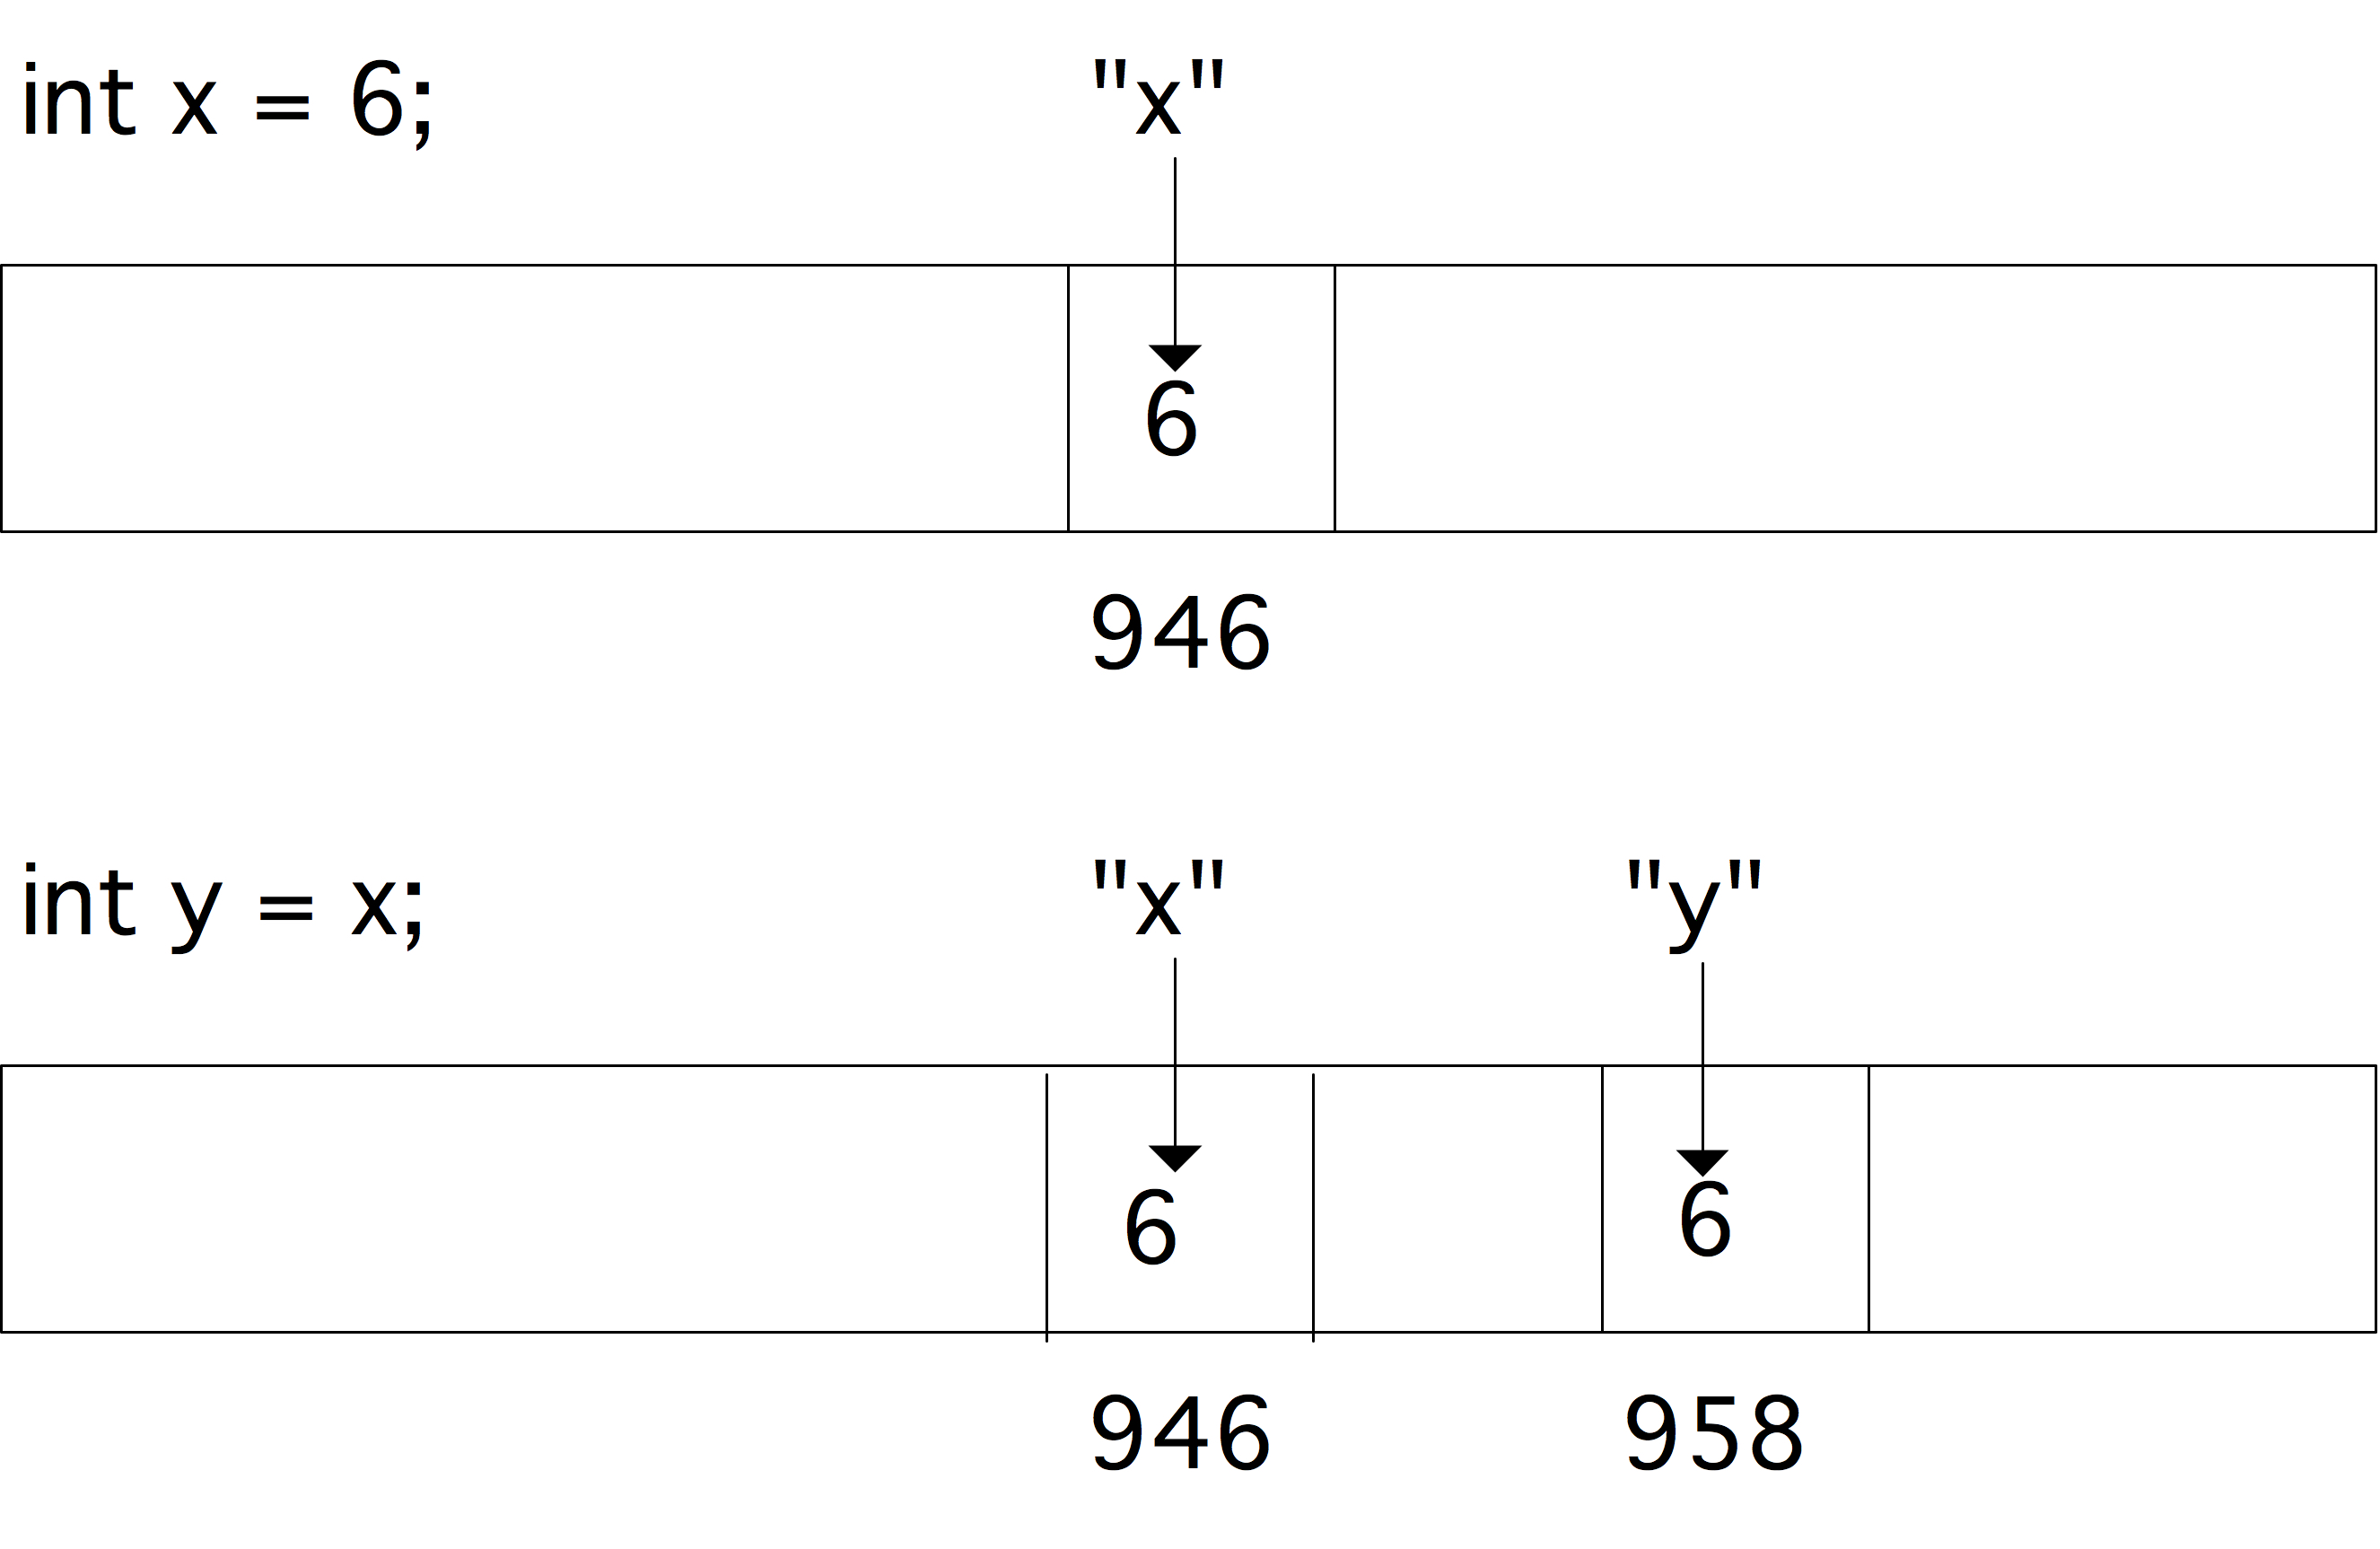
\includegraphics[scale=.1]{intstar1}
\end{block}

\begin{block}{illustration}
  \label{sl:deref-pic}
  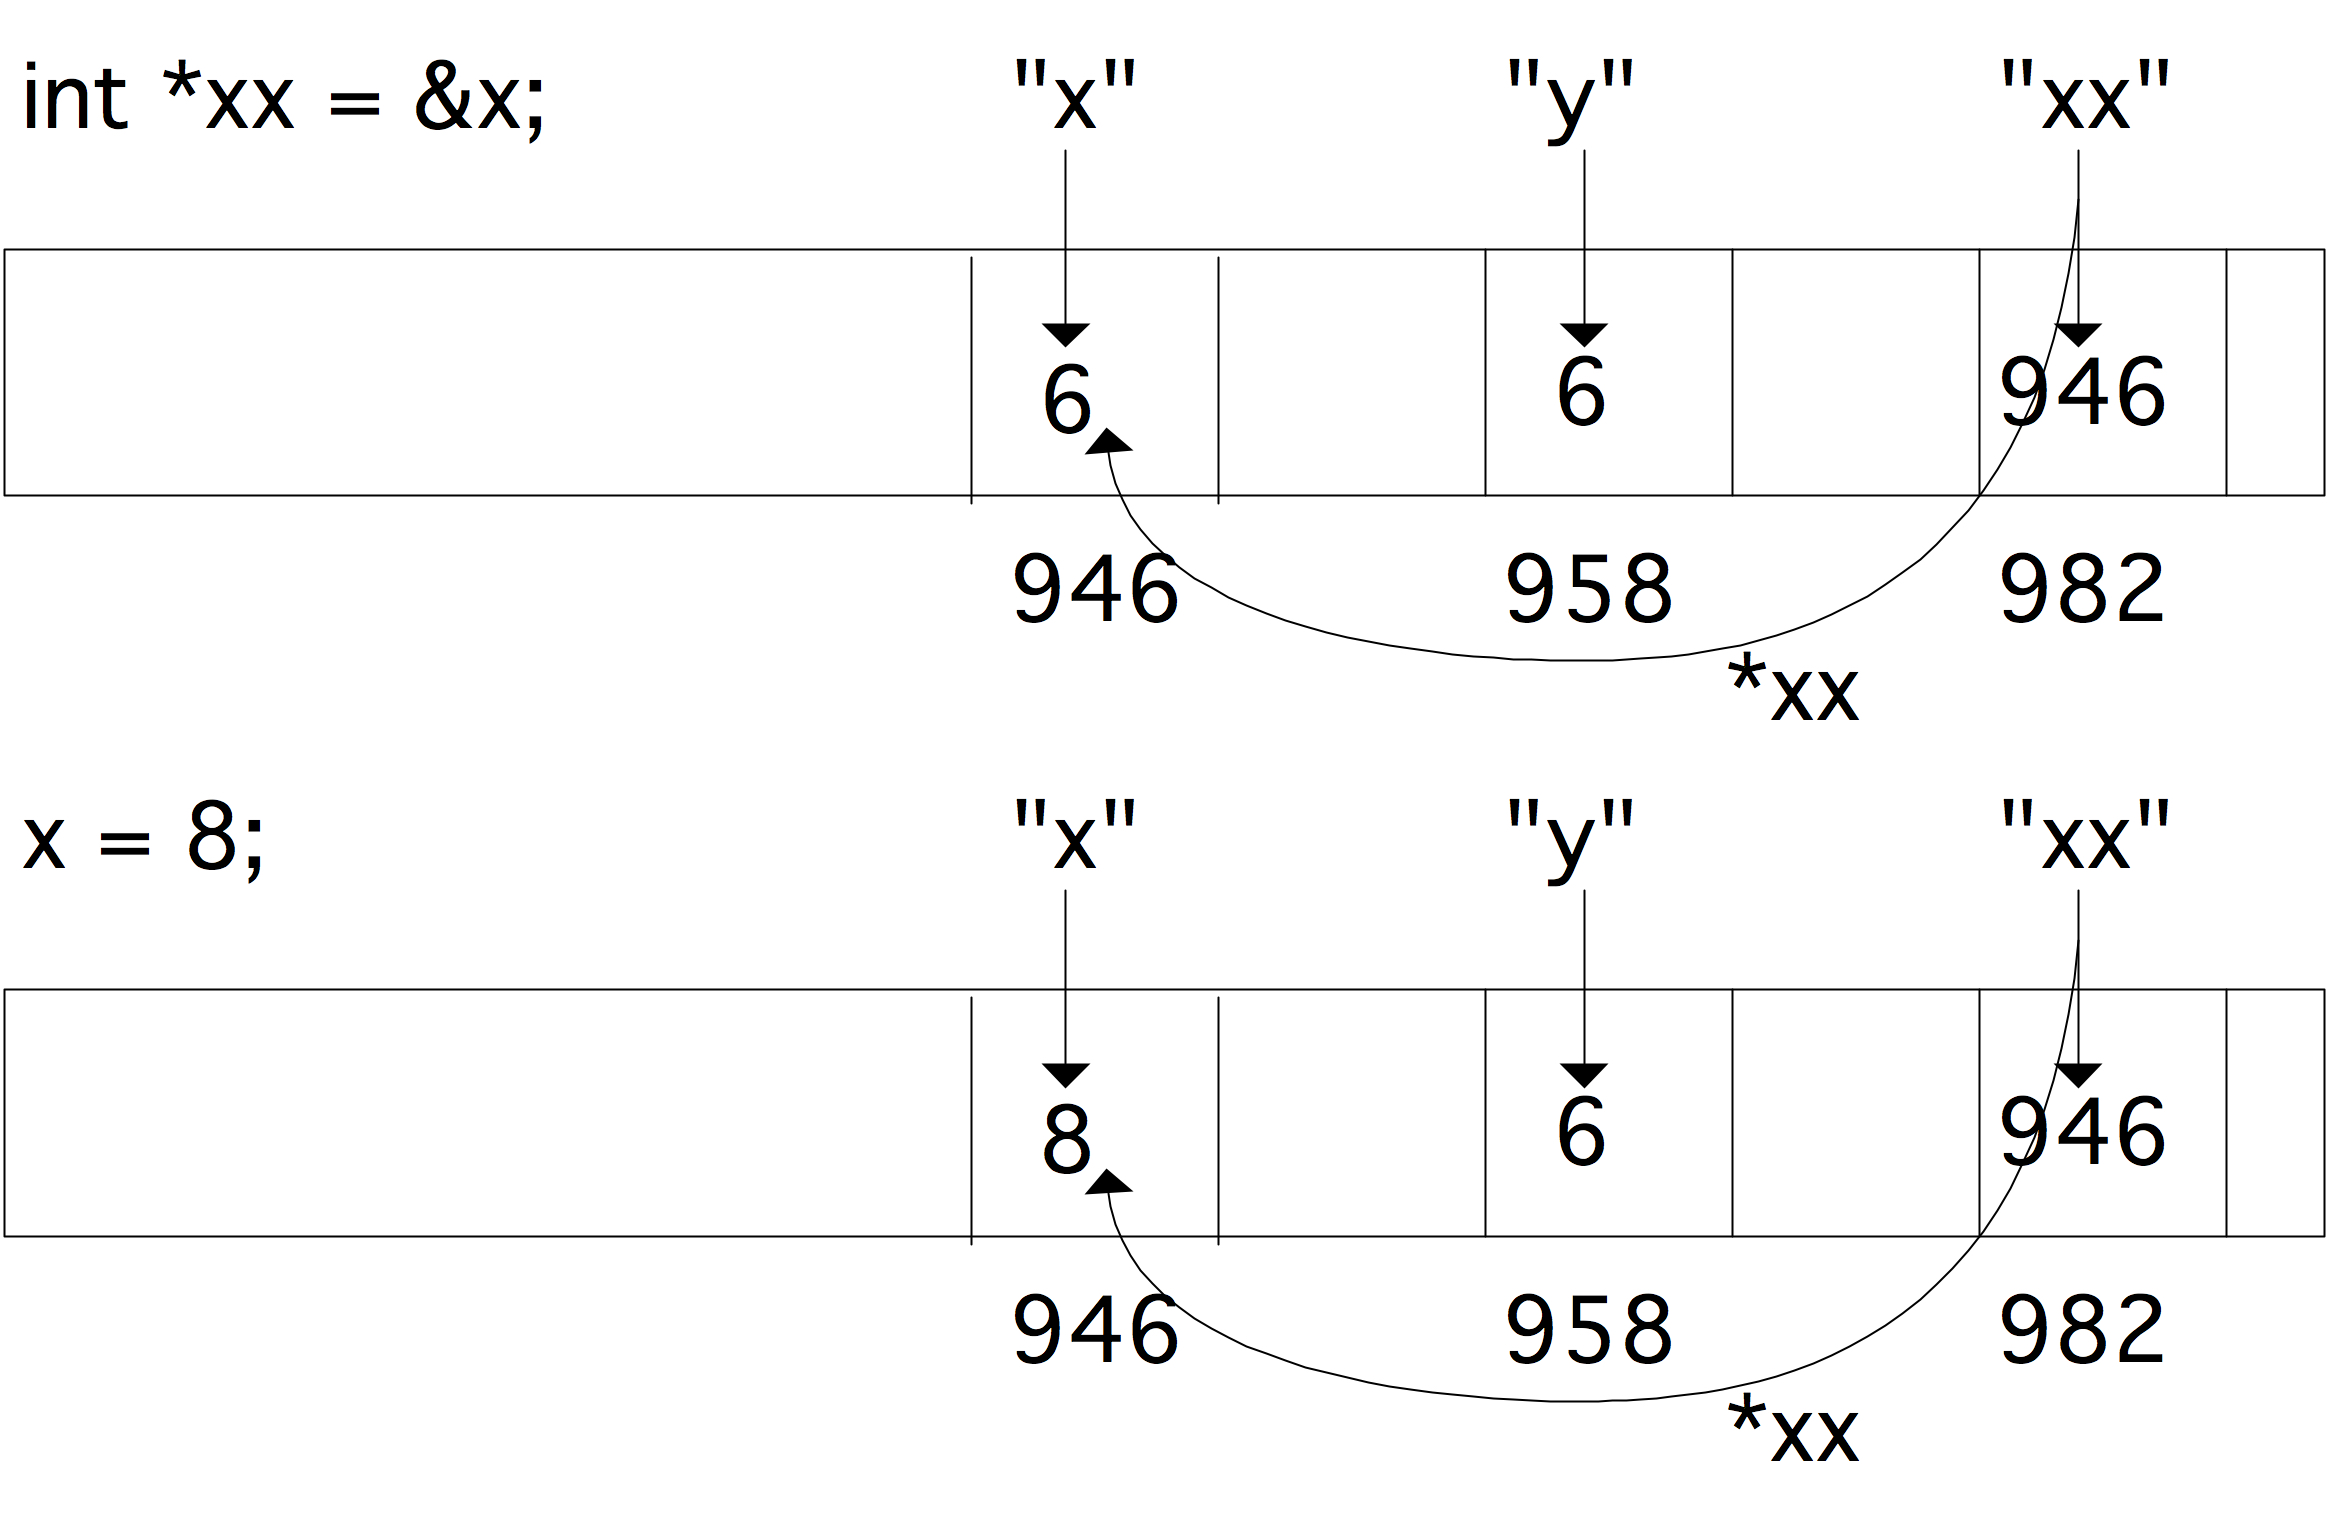
\includegraphics[scale=.1]{intstar2}
\end{block}

\begin{itemize}
\item \lstinline{addr} is the address of~\lstinline{i}.
\item You set \lstinline{i} to~5; nothing changes about \lstinline{addr}. This has the
  effect of writing \lstinline{5} in the memory location of~\lstinline{i}.
\item The first \lstinline{cout} line dereferences \lstinline{addr}, that is, looks up
  what is in that memory location.
\item Next you change \lstinline{i} to~\lstinline{6}, that is, you write \lstinline{6} in its
  memory location.
\item The second \lstinline{cout} looks in the same memory location as before,
  and now finds~\lstinline{6}.
\end{itemize}

The syntax for declaring a pointer-to-sometype allows for a small
variation, which indicates the two way you can interpret such a declaration.

\begin{block}{Star stuff}
  \label{sl:starstuff}
  Equivalent:
  \begin{itemize}
  \item \lstinline{int* addr}: \lstinline{addr} is an int-star, or
  \item \lstinline{int *addr}: \lstinline{*addr} is an int.
  \end{itemize}
\end{block}

The notion \lstinline{int* addr} is equivalent to \lstinline{int *addr}, and
semantically they are also the same: you could say that \lstinline{addr} is an
int-star, or you could say that \lstinline{*addr} is an int.

\Level 0 {Arrays and pointers}
\label{sec:arraypointer}

In section~\ref{sec:staticarray} you saw the treatment of static
arrays in~C++. Examples such as:
%
\verbatimsnippet{arraypass}
%
show that, even though an parameters are normally passed by value, that is
through copying, array parameters can be altered. The reason for this
is that there is no actual array type, and what is passed is a pointer
to the first element of the array. So arrays are still passed by
value, just not the `value of the array', but the value of its
location.

So you could pass an array like this:
%
\verbatimsnippet{arraypassstar}

\begin{block}{Array and pointer equivalence}
  \label{sl:array-pointer}
  Array and memory locations are largely the same:
  %
  \snippetwithoutput{arrayaddr}{pointer}{arrayaddr}
\end{block}

\begin{block}{Array passing to function}
  \label{sl:array-function}
  When an array is passed to a function,
  it behaves as an address:
  %
  \snippetwithoutput{arraypass}{pointer}{arraypass}

  Note that these arrays don't know their size, so
  you need to pass it.
\end{block}

\begin{block}{Dynamic allocation}
  \label{sl:newstar}
  You can dynamically reserve memory with \lstinline{new}, which gives
  a something-star:
\begin{lstlisting}
double *x;
x = new double[27];
\end{lstlisting}
\end{block}

The \lstinline{new} operator is only for C++: 
in C you would use  \indexcdef{malloc} to dynamically allocate memory.
The above example would become:
\begin{lstlisting}
double *x;
x = (double*) malloc( 27 * sizeof(double) );
\end{lstlisting}
Note that \lstinline{new} takes the number of elements, and deduces
the type (and therefore the number of bytes per element) from the
context; \lstinline{malloc} takes an argument that is the number of
bytes. The \indexcdef{sizeof} operator then helps you in
determining the number of bytes per element.

\Level 0 {Pointer arithmetic}

\begin{block}{Pointer arithmetic}
  \indextermbus{pointer}{arithmetic} uses the size of the objects it
  points at:
\begin{lstlisting}
double *addr_of_element = array;
cout << *addr_of_element;
addr_of_element = addr_of_element+1;
cout << *addr_of_element;
\end{lstlisting}
Increment add size of the array element, 4~or~8 bytes, not~one!
\end{block}

\begin{exercise}
  Write a subroutine that sets the i-th element of an array, but using
  pointer arithmetic: the routine should not contain any square brackets.
\end{exercise}

\Level 0 {Multi-dimensional arrays}

\begin{block}{Multi-dimensional arrays}
  \label{sl:static-multi}
After
\begin{lstlisting}
double x[10][20];
\end{lstlisting}
a row \lstinline{x[3]} is a \lstinline{double*}, so is \lstinline{x} a \lstinline{double**}?

Was it created as:
\begin{lstlisting}
double **x = new double*[10];
for (int i=0; i<10; i++)
  x[i] = new double[20];
\end{lstlisting}
No: multi-d arrays are contiguous.
\end{block}

\Level 0 {Parameter passing}
\index{C!parameter passing|(}

\begin{block}{C++ pass by reference}
  \label{sl:cpp-pass-ref}
  C++ style functions that alter their arguments:
\begin{lstlisting}
void inc(int &i) {
  i += 1;
}
int main() {
  int i=1;
  inc(i);
  cout << i << endl;
  return 0;
}
\end{lstlisting}
\end{block}

\begin{block}{C-style pass by reference}
  \label{sl:c-pass-ref}
  In C you can not pass-by-reference like this. Instead, you pass the
  address of the variable~\lstinline{i} by value:
\begin{lstlisting}
void inc(int *i) {
  *i += 1;
}
int main() {
  int i=1;
  inc(&i);
  cout << i << endl;
  return 0;
}
\end{lstlisting}
Now the function gets an argument that is a memory address: \lstinline{i}~is
an int-star. It then increases \lstinline{*i}, which is an int variable, by one.
\end{block}

Note how again there are two different uses of the ampersand
character.  While the compiler has no trouble distinguishing them, it
is a little confusing to the programmer.

\begin{exercise}
  \label{ex:c-star-swap}
  Write another version of the \lstinline{swap} function:
\begin{lstlisting}
void swap( /* something with i and j */ {
  /* your code */
}
int main() {
  int i=1,j=2;
  swap( /* something with i and j */ );
  cout << "check that i is 2: " << i << endl;
  cout << "check that j is 1: " << i << endl;
  return 0;
}
\end{lstlisting}
Hint: write C++ code, then insert stars where needed.
\end{exercise}

\Level 1 {Allocation}

In section~\ref{sec:staticarray} you learned how to create arrays that
are local to a scope:

\begin{block}{Problem with static arrays}
  \label{sl:no-static-alloc}
  Create an array with size depending on something:
\begin{lstlisting}
if ( something ) {
  double ar[25];
} else {
  double ar[26];
}
ar[0] = // there is no array!
\end{lstlisting}
This Does Not Work
\end{block}

The array \lstinline{ar} is created depending on if the condition is true, but
after
the conditional it disappears again. The mechanism of using
\indexc{new} (section~\ref{sec:cnew}) allows you to allocate
storage that transcends its scope:

\begin{block}{Allocation, C vs C++}
  \label{sl:c-array-malloc}
  C allocates in bytes:
\begin{lstlisting}
double *array;
array  = (double*) malloc( 25*sizeof(double) );
\end{lstlisting}
C++ allocates an array:
\begin{lstlisting}
double *array;
array  = new double[25];
\end{lstlisting}
Don't forget:
\begin{lstlisting}
free(array); // C
delete array; // C++
\end{lstlisting}
\end{block}

\begin{block}{Declaration and allocation}
  \label{sl:c-array-new}
Now dynamic allocation:
\begin{lstlisting}
double *array;
if (something) {
  array = new double[25];
} else {
  array = new double[26];
}
\end{lstlisting}
Don't forget:
\begin{lstlisting}
delete array;
\end{lstlisting}
\end{block}

\begin{block}{Memory leak1}
  \label{sl:leak1}
\begin{lstlisting}
void func() {
  double *array = new double[large_number];
  // code that uses array
}
int main() {
  func();
};
\end{lstlisting}
\begin{itemize}
\item
  The function allocates memory
\item After the function ends, there is no way to get at that memory
\item $\Rightarrow$ \indextermbusdef{memory}{leak}.
\end{itemize}

\end{block}

\begin{block}{Memory leaks}
  \label{sl:leak2}
\begin{lstlisting}
for (int i=0; i<large_num; i++) {
  double *array = new double[1000];
  // code that uses array
}
\end{lstlisting}
  Every iteration reserves memory, which is never released:
  another \indextermbus{memory}{leak}.

  Your code will run out of memory!
\end{block}

\begin{block}{De-allocation}
  \label{sl:c-array-del}
  Memory allocated with \lstinline{malloc}~/ {new}
  does not disappear when you leave a
  scope. Therefore you have to delete the memory explicitly:
\begin{lstlisting}
free(array);
delete(array);
\end{lstlisting}
The C++ \lstinline{vector} does not have this problem, because it obeys scope rules.
\end{block}

\begin{block}{Stop using C!}
  \label{sl:no-c-malloc}
  No need for \lstinline{malloc} or \lstinline{new}
  \begin{itemize}
  \item Use \lstinline{std::string} for character arrays, and
  \item \lstinline{std::vector} for everything else.
  \end{itemize}
  No performance hit if you don't dynamically alter the size.
\end{block}

\Level 2 {Malloc}

The keywords \lstinline{new} and \lstinline{delete} are in the spirit of C~style
programming, but don't exist in~C. Instead, you use
\indexc{malloc}, which creates a memory area with a size
expressed in bytes. Use the function \indexc{sizeof} to translate
from types to bytes:

\begin{block}{Allocation in C}
\begin{lstlisting}
int n;
double *array;
array = malloc( n*sizeof(double) );
if (!array)
  // allocation failed!
\end{lstlisting}
\end{block}

\Level 2 {Allocation in a function}

The mechanism of creating memory, and assigning it to a `star'
variable
can be used to allocate data in a function and
return it from the function.

\begin{block}{Allocation in a function}
\begin{lstlisting}
void make_array( double **a, int n ) {
  *a = new double[n];
}
int main() {
  double *array;
  make_array(&array,17);
}
\end{lstlisting}
\end{block}

Note that this requires a `double-star' or `star-star' argument:
\begin{itemize}
\item The variable \lstinline{a} will contain an array, so it needs to be of
  type \lstinline{double*};
\item but it needs to be passed by reference to the function, making
  the argument type~\lstinline{double**};
\item inside the function you then assign the new storage to the
  \lstinline{double*} variable, which is~\lstinline{*a}.
\end{itemize}
Tricky, I~know.

\Level 1 {Use of \texttt{new}}
\label{sec:cnew}

\prerequisite{\ref{sec:arraypointer}}

There is a dynamic allocation mechanism that is much inspired by
memory management in~C. Don't use this as your first choice.

Use of \indexc{new} uses the 
equivalence of array and reference.
%
\verbatimsnippet{arrayfromfunc}

Since this is not scoped, you have to free the memory yourself:
%
\verbatimsnippet{arrayinclass}

Notice how you have to remember the array length yourself? This is all
much easier by using a \lstinline{std::vector}. See
\url{http://www.cplusplus.com/articles/37Mf92yv/}.

The \indexc{new} mechanism is a cleaner variant of \indexc{malloc},
which was the dynamic allocation mechanism in~C. Malloc is still
available, but should not be used. There are even very few legitimate
uses for \lstinline{new}.

\index{C!parameter passing|)}

\Level 0 {Memory leaks}
\label{sec:memleak}

Pointers can lead to a problem called \indextermdef{memory leaking}:
there is memory that you have reserved, but you have lost the ability
to access it.

In this example:
\begin{lstlisting}
double *array = new double[100];
// ...
array = new double[105];
\end{lstlisting}
memory is allocated twice. The memory that was allocated first is
never release, because in the intervening code another pointer to it
may have been set. However, if that doesn't happen, the memory is both
allocated, and unreachable. That's what memory leaks are about.

\Level 0 {Const pointers}

A pointer can be constant in two ways:
\begin{enumerate}
\item It points to a block of memory, and you can not change where
  it points.
\item What it points to is fixed, and the contents of that memory can
  also not be altered.
\end{enumerate}

To illustrate the non-const behavior:
%
\snippetwithoutput{cptrinc}{pointer}{starconst1}

A pointer that is constant in the first sense:
%
\verbatimsnippet{cptrconst}

You can also make a pointer to a constant integer:
%
\verbatimsnippet{cptrtoconst}

\index{C!pointer|)}
